% *******************************************************
% SUPPRESS WARNINGS
% *******************************************************
\RequirePackage{silence}
\WarningFilter{scrbook}{Usage of package `titlesec'}
\WarningFilter{titlesec}{Non standard sectioning command detected}

% *******************************************************
% DOCUMENT FRONT MATTER START
% *******************************************************
\documentclass[11pt,twoside,openright,titlepage,
  headinclude,footinclude,BCOR=5mm,
  numbers=noenddot,cleardoublepage=empty,
  tablecaptionabove, dottedtoc,
  bibliography=totoc]{scrreprt}
\usepackage{subfig}
\usepackage[eulerchapternumbers, subfig, beramono, eulermath, pdfspacing]{classicthesis} 
\usepackage{arsclassica}
\usepackage{amsmath}
\usepackage{amssymb}
\usepackage{graphicx}
\usepackage{booktabs}
\usepackage[utf8]{inputenc}
\usepackage[T1]{fontenc}
\usepackage{pdfpages}
\usepackage{titlesec}
\usepackage{titletoc}
\usepackage[norsk,american]{babel}
\usepackage[paperwidth=17cm, paperheight=24cm, margin=2.5cm]{geometry}
\usepackage[cam,a4,center,pdflatex]{crop}

% *******************************************************
% ADDITIONAL PACKAGES
% *******************************************************

% *******************************************************
% REFERENCE PACKAGES
% *******************************************************
  \usepackage[authoryear]{natbib}
  \bibliographystyle{plainnat}

% *******************************************************
% DEFINE VARIABLES
% *******************************************************
\newcommand{\Name}{Raju Rimal}
\newcommand{\Title}{Exploration of Multi-Response Multivariate Methods}
\newcommand{\Location}{\spacedlowsmallcaps{Ås}}
\newcommand{\Year}{2019}
\newcommand{\Month}{Apr}
\newcommand{\Date}{\Year, \Month}
\newcommand{\docsite}{\url{https://therimalaya.github.com/thesis}}
\newcommand{\Subtitle}{}
\newcommand{\email}{\mail{raju.rimal@nmbu.no}}
\newcommand{\homepage}{\url{https://www.mathatistics.com/}}
\newcommand{\Affiliation}{Biostatistics\\
Dept. of Chemistry, Biotechnology and Food Science\\
Norwegian University of Life Sciences}
\newcommand{\Faculty}{}
\newcommand{\Group}{}
\newcommand{\alttitle}{Utforskning av multi-respons multivariate metoder}

% *******************************************************
% CUSTOMIZATIONS
% *******************************************************
\newcommand{\mail}[1]{\href{mailto:#1}{\texttt{#1}}}
\titlecontents{part}[0pt]{\pagebreak}{}{\Large\MakeTextUppercase}{}
\titleformat{\part}[display]
  {\normalfont\centering\Large}%
  {\thispagestyle{empty}\partname~\MakeTextUppercase{\thepart}}{1em}%
  {\color{Maroon}\spacedallcaps}
\providecommand{\tightlist}{%
  \setlength{\itemsep}{0pt}\setlength{\parskip}{0pt}}
\DeclareTOCStyleEntry[beforeskip=3pt]{tocline}{section}

% *******************************************************
% DOCUMENT BEGIN
% *******************************************************
\begin{document}
\pagenumbering{Roman}
\pagestyle{plain}

% *******************************************************
% Title Front
% *******************************************************
\begin{titlepage}
  \pdfbookmark{Titlepage}{Titlepage}
  \begin{center}
    \large \sffamily
    \bigskip
    {\huge\spacedlowsmallcaps{\Title} \\}
    \bigskip
    {\large{\alttitle}} \\
    \vfill
    {\Large\spacedlowsmallcaps{Doctor of Philosophy (PHD) Thesis}} \\
    \bigskip
    {\Large{\spacedlowsmallcaps\Name}} \\
    \vfill
    {\normalsize \Affiliation}
    \vfill
    {\normalsize \Location, \Year \\}
    \vfill
              \newcommand{\logowidth}{0.6\linewidth}
          
\includegraphics[width=\logowidth]{Logo.pdf} \\
        \vfill
    {\normalsize
      Thesis Number: 1234:56\\
      ISSN:  1234-5678\\
      ISBN:  123-45-678-1234-5\\
    }
  \end{center}
\end{titlepage}

% *******************************************************
% Title Back
% *******************************************************
\thispagestyle{empty}
\hfill \vfill
\noindent
\textit{The goal is to turn data into information, and information into insight.}\\
\spacedlowsmallcaps{- Carly Fiorina, former CEO of Hewlett-Packard}
\vfill
\noindent
{\textbf{Supervisors:}} \\
Professor \textit{Solve Sæbø}\\
Prorector\\
Norwegian University of Life Sciences\\
Ås, Norway\\
\medskip\\
Associate Professor \textit{Trygve Almøy}\\
Dept. of Chemistry, Biotechnology and Food Science\\
Norwegian University of Life Sciences\\
Ås, Norway\\
\medskip\\
\bigskip \\
\noindent
\textit{\Title} \\
{\spacedlowsmallcaps{PhD Thesis, \Date\,\, \textcopyright\, \Name}} \\
\bigskip \\
\noindent{\spacedlowsmallcaps{Website}}: \\
\docsite \\
\medskip
\noindent{\spacedlowsmallcaps{E-mail}}: \\
\email
\vspace{1cm}
\hrule
\bigskip
\noindent This thesis is prepared with \texttt{ArsClassica} {\LaTeX} template with \texttt{pandoc} and r-package \texttt{bookdown}.
% \begin{flushright}source: \url{https://therimalaya.github.com/thesis}\end{flushright}
\pagestyle{scrheadings} 

% *******************************************************
% ABSTRACT
% *******************************************************

% *******************************************************
% SUMMARY
% *******************************************************
\begingroup
\pdfbookmark{Summary}{Summary}
\addchap{Summary}
A linear regression model defines a linear relationship between two or
more random variables. The random variables that depend on other random
variables are often called response variables and the independent random
variables are called predictor variables. In most cases not all
variation is relevant for regression, i.e.~only a certain amount of the
variation in the predictors is relevant and only so for a part of the
variation in the response. This leads to a reduction of the linear
regression model where one can imagine a subspace of the space spanned
by the predictor variables that contains all the relevant information
for a subspace of the space spanned by the response variables.

In this thesis we attempt to compare some new methods which are based on
the envelope model and some established methods such as principal
components regression (PCR) and partial least squares regression (PLS).
The comparison tests these methods on their performance of producing
minimum prediction and estimation error while modelling data simulated
with specifically designed properties. For the simulation we have also
created an R-package called \texttt{simrel} with a web interface.

A simulation model for a multi-response multivariate linear model, on
which the simulation tool is based, is discussed in the first paper.
This paper prepares a basic foundation for the simulations with the
concept of reduction of regression models. The second paper discusses
the similarities of the envelope, PCR and PLS population models. This
paper compares the prediction performance of several multivariate
methods using a model with a single response.

The final two papers make an extensive investigation evaluating the
prediction and estimation performance of established (PCR, PLS1 and
PLS2) and newly developed envelope based (Xenv and Senv) methods.
Unsurprisingly the study found that not one method dominates in all
situations, but their performance depend on the properties of the data
they model. However, the envelope based methods have shown remarkable
performance in many cases, both in prediction and estimation. The study
also recommend researchers to use and evaluate the envelope methods.


\KOMAoptions{open=left}
\begin{otherlanguage}{norsk}
\pdfbookmark{Sammendrag}{Sammendrag}
\addchap{Sammendrag}
En lineær regresjonsmodell definerer et lineært forhold mellom to eller
flere tilfeldige variabler. De tilfeldige variablene som er avhengige av
andre tilfeldige variabler, kalles ofte responsvariabler, og de
uavhengige tilfeldige variablene kalles prediktorvariabler. I de fleste
tilfeller er ikke all variasjon relevant for regresjon, dvs. bare en
viss mengde variasjonen i prediktorene er relevante, og bare for en del
av variasjonen i responsen. Dette fører til en reduksjon av den lineære
regresjonsmodellen der man kan forestille seg et underrom av rommet som
spennesut av prediktorvariablene som inneholder all relevant informasjon
for et underrom av rommet spent ut av responsvariablene.

I denne avhandlingenprøver vi å sammenligne noen nye metoder som er
basert på Envelopemodellen og noen etablerte metoder som principal
komponent regresjon (PCR) og partiell minste kvadraters regresjon (PLS).
Sammenligningen tester disse metodene på deres ytelse til å produsere
minimum prediksjon- og estimeringsfeil, mens modelleringsdata simuleres
med spesielt designede egenskaper. For simuleringen har vi også laget en
R-pakke kalt \texttt{simrel} med et webgrensesnitt.

En simuleringsmodell for multirespons, multivariat lineær modell, som
simuleringsverktøyet bygger på, diskuteres i den første artikkelen.
Denne artikkelen utarbeider et grunnleggende fundament for simuleringene
basert på konseptet om reduksjon av regresjonsmodeller. Den andre
artikkelen diskuterer likhetene i Envelope-, PCR- og
PLS-populasjonsmodellene. Denne artikkelen sammenligner
prediksjonsytelsen til flere multivariate metoder ved bruk av en modell
med en enkelt respons.

De to siste artiklene gir en grundig evaluering av prediksjons- og
estimeringsegenskapene til etablerte metoder (PCR, PLS1 og PLS2) og
nyutviklede envelope-baserte metoder (Xenv og Senv). Ikke uventet fant
studien at det ikke finnes en enkelt metode som dominerer i alle
situasjoner, men resultatene deres avhenger av egenskapene til dataene
de modellerer. Imidlertid har envelope-baserte metoder vist
bemerkelsesverdig resultater i mange tilfeller, både når det gjelder
prediksjon og estimering. Studien anbefaler også forskere å bruke og
evaluere envelope-metodene.

\end{otherlanguage}{norsk}
\KOMAoptions{open=right}
\endgroup

% *******************************************************
% ACKNOWLEDGMENT
% *******************************************************
\pdfbookmark{Acknowledgments}{Acknowledgments}
\begingroup
\cleardoublepage
\addchap{Acknowledgment}
First and foremost, I am indebted to my supervisor Solve Sæbø who picked
me up from nowhere and brought me into a scientific community by giving
me a chance to pursue this degree. His inspiration and encouragement
have been an essential element in the course of this journey. I am
grateful to my co-supervisor Trygve Almøy for being a mentor, a friend,
a colleague, and a guardian and guiding and supporting me throughout
this period. He has always been there for me with my frustration and
excitement.

I am forever grateful to my father Narayan Prasad Rimal and mother
Bhagawati Rimal for their continuous support and encouragement. Their
belief in me and push for my education have shined the light in my hard
and easy times. I am also thankful to my dear wife Junali Chhetri who
has inspired me every step of my life and help me to better understand
myself. And of course, a thank goes to my beloved son Nirvan Rimal who
has understood my busy time during this study.

I would also like to thank Professor Inge Helland for his insight,
suggestion and comment on many mathematical problems on various
statistical methods presented in the thesis.

Last, but importantly, my thank goes to the Biostatistics group with
whom I have collected beautiful memories. Thanks to all the members of
the group from past and present who have always made my stay at NMBU
happy, festive and full of joy.

\endgroup

% *******************************************************
% PREFACE
% *******************************************************
\pdfbookmark{Preface}{Preface}
\begingroup
\cleardoublepage
\addchap{Preface}
This thesis is a part of Doctor of Philosophy (PhD) study. The first
part of the thesis constitute a gentle introduction to the objective of
the study and some of its background. This is followed by the summary of
individual research paper on which this thesis is based on. The
discussion section tries to bind the finding from theses papers. The
final chapter will discuss the limitations and future prospect of the
study. The second part contains all the papers attached.

An R-package called \texttt{simrel} is available as part of the first
paper included in this thesis. The package lets users simulated data
from a multi-response linear model. The package can be installed from
R-package repository CRAN or from GitHub. In addition, a web application
that gives users a graphical user interface for the package is also
available from GitHub. All the results and the documentations of the
research can be reproduced from the codes in GitHub repository with
software and packages required installed. In addition, one can use
docker image together with the code for reproducing the thesis together
with all included papers. All related resources are listed in the final
chapter.

\endgroup

% *******************************************************
% INCLUDE ANYTHING BEFORE
% *******************************************************

% *******************************************************
% Contents
% *******************************************************
\cleardoublepage
\phantomsection
\pdfbookmark{\contentsname}{tableofcontents}
\setcounter{tocdepth}{2}
\begingroup 
  \let\clearpage\relax
  \let\cleardoublepage\relax
    \tableofcontents
\endgroup
\markboth{\spacedlowsmallcaps{\contentsname}}
{\spacedlowsmallcaps{\contentsname}} 

\begingroup
\cleardoublepage
\listoftables
\vfill
\let\clearpage\relax
\let\cleardoublepage\relax

\listoffigures
\vfill
\endgroup

\begingroup 
  \let\clearpage\relax
  \let\cleardoublepage\relax
\endgroup

\cleardoublepage

% *******************************************************
% BODY START
% *******************************************************

\pagenumbering{arabic}

\hypertarget{introduction}{%
\chapter{Introduction}\label{introduction}}

As a consequence of the development in the technology and computing power, data science discipline has emerged from the explosion of data. Extracting information from this chaotic heap of data has become another problem. Many statistical and machine learning tools are being devised for this purpose. However the difference in the approach, these methods target the problem, makes them distinct and useful to deal with certain aspect of the data. Most of these problems lie in identifying the relationship between variables. This thesis confined itself in the exploration of linear relationship where a set of independent variables called predictor variables affect another set of dependent variables called response variables. Normally only subspace of predictor variables are relevant for a subspace of response variables to define its linear relationship. This brings to the concept of relevant and irrelevant space. Methods like Principal Components Regression (PCR), Partial Least Squares (PLS) and many other variants of PLS has leveraged this concept and are serving as a prime tool in many discipline, most notably chemometrics. A relatively new methods called envelopes has used this concept of dimension reduction such that only the relevant (material) part in both response and predictors can be used to estimate the underlying linear model. Although the underlying population model is similar in these methods, they estimate the model parameter differently. Evaluation of these methods is crucial in order to understand their pros and cons on dataset with certain properties. This thesis will explore some of these methods and access their estimative and predictive strength and weaknesses through both simulated and real datasets. This exploration adds a reference for researchers and motivates them for using different methods based on the properties of the data they are working on.

This study is exploratory in nature where we assess and compare different multi-response multivariate methods but most importantly study their interaction with the properties of the data. The properties include the correlation between predictor variables, the position of principal components of predictor variables (predictor components) that are relevant for certain principal components of response variables (response components), the amount of correlation between the response variables and the number of predictor variables. The effect of correlation structure of response matrix is less explored and it is expected to add some light on how similar and how different the methods are in terms of modelling this structure. In order to simulate data with these properties varying at different levels, we have created an R-package called \texttt{simrel} which is an extension of the previous version of it introduced by \citet{saebo2015simrel} to incorporate multiple response.

\hypertarget{background}{%
\section{Background}\label{background}}

In the following few subsection, I will discuss few related topics in this thesis. These topics are extensively used in all the papers which are summarized in next chapter.

\hypertarget{multivariate-linear-regression-model}{%
\subsection{Multivariate Linear Regression Model}\label{multivariate-linear-regression-model}}

A model that linearly relates a random variable \(\mathbold{y}\) consists of \(m\) response variables with another random variable \(\mathbold{x}\) consists of \(p\) predictor variables through regression coefficient \(\boldsymbol{\beta}\) is often written as,

\begin{equation}
\mathbold{y} = \boldsymbol{\mu}_y + \boldsymbol{\beta}^t\left(\mathbold{x} - \boldsymbol{\mu}_x\right) + \boldsymbol{\varepsilon}
\end{equation}
where \(\boldsymbol{\varepsilon} \sim \textsf{N}\left(\mathbold{0}, \boldsymbol{\Sigma}_{y|x}\right)\), \(\boldsymbol{\mu}_y\) is the mean vector of \(\mathbold{y}\) and \(\boldsymbol{\mu}_x\) is the mean vector of \(\mathbold{x}\).

Here the regression coefficient \(\boldsymbol{\beta} = \boldsymbol{\Sigma}_{xx}^{-1}\boldsymbol{\Sigma}_{xy}\)
- A linear model
- Linear relationship model

\hypertarget{relevant-space-and-relevant-components}{%
\subsection{Relevant Space and Relevant Components}\label{relevant-space-and-relevant-components}}

\begin{itemize}
\tightlist
\item
  Connection to relevant space
\item
  How relevant space is connected to relevant component and dimension reduction
\item
  Concept linked to simrel and various methods
\end{itemize}

\hypertarget{estimation-and-prediction}{%
\subsection{Estimation and Prediction}\label{estimation-and-prediction}}

\begin{itemize}
\tightlist
\item
  What is the difference between estimation and prediction
\item
  How large estimation error can also result in close prediction
\item
  What have we used in these papers for comparison
\end{itemize}

\hypertarget{multivariate-analysis-of-variance}{%
\subsection{Multivariate Analysis of Variance}\label{multivariate-analysis-of-variance}}

\begin{itemize}
\tightlist
\item
  What is ANOVA in multi-response setting
\item
  Why is it different from regular ANOVA
\item
  How we have used this method in our study
\item
  What statistic we have used for comparison
\end{itemize}

\hypertarget{previous-studies}{%
\section{Previous Studies}\label{previous-studies}}

\begin{itemize}
\tightlist
\item
  Previous similar studies
\item
  Mostly used the methods developers
\item
  Connection with data properties in an experimental manner is not explored properly and comprehensively
\item
  Effect on multi-response model and the effect of correlation structure on the methods is not studied for these methods to our knowledge
\end{itemize}

\hypertarget{simulation-and-experimental-design}{%
\section{Simulation and Experimental Design}\label{simulation-and-experimental-design}}

\begin{itemize}
\tightlist
\item
  Different papers have different design
\item
  Last two papers have similar design as the fourth paper extends the third
\item
  Following factors and their interaction is studied,

  \begin{itemize}
  \tightlist
  \item
    Low and High multicollinearity
  \item
    Position of predictor components that are relevant for specific response components
  \item
    Number of predictor variables
  \item
    Low to High correlation between response variables
  \end{itemize}
\end{itemize}

The exploration and findings of the papers are discussed in brief in next chapter.

\hypertarget{paper-summary}{%
\chapter{Paper Summary}\label{paper-summary}}

\hypertarget{paper-1-a-tool-for-simulating-multi-response-linear-model-data}{%
\section{Paper 1: A tool for simulating multi-response linear model data}\label{paper-1-a-tool-for-simulating-multi-response-linear-model-data}}

\begin{itemize}
\tightlist
\item
  Extend the simulation tool introduced by \ldots solve2015simrel\ldots{} for multi-response simulation
\item
  Gives the mathematical formulation for the simulation
\item
  Makes basic comparison on various multivariate methods using both simulated and real data
\item
  Shows that \ldots{}
\end{itemize}

\hypertarget{paper-2-model-and-estimators-for-partial-least-squares-regression}{%
\section{Paper 2: Model and estimators for partial least squares regression}\label{paper-2-model-and-estimators-for-partial-least-squares-regression}}

\begin{itemize}
\tightlist
\item
  The paper shows the similarity of population model of PCR, PLS and envelope in predictors
\item
  My contribution on the paper is on the example of a comparative study with single response with both simulated and real data
\item
  BayesPLS showed better performance with few fallback such as crashing, time consuming and lack of method for multi-response model
\item
  It also showed that \ldots{} on the prediction performance
\end{itemize}

\hypertarget{paper-3-comparison-of-multi-response-prediction-methods}{%
\section{Paper 3: Comparison of Multi-response Prediction Methods}\label{paper-3-comparison-of-multi-response-prediction-methods}}

\begin{itemize}
\tightlist
\item
  This paper extends the comparative study on both of the previous paper
\item
  Here only methods based on relevant space is considered for comparison
\item
  A small modification in the envelope methods is made as the methods is based on maximum likelihood and can not be fitted on \(p>>n\) case.
\item
  The results showed that \ldots{}
\end{itemize}

\hypertarget{paper-4-comparison-of-multi-response-estimation-methods}{%
\section{Paper 4: Comparison of Multi-response Estimation Methods}\label{paper-4-comparison-of-multi-response-estimation-methods}}

\begin{itemize}
\tightlist
\item
  Since good prediction not always results in good estimation, this paper continue the exploration of Paper3 for the estimation performance of the methods
\item
  The same data is used with the similar modification in envelope methods
\item
  The interaction of methods and the design on the basis of error is studied with MANOVA in both Paper3 and Paper4
\end{itemize}

\hypertarget{discussions-conclusions-and-future-perspectives}{%
\chapter{Discussions, Conclusions and Future Perspectives}\label{discussions-conclusions-and-future-perspectives}}

\hypertarget{discussions-and-conclusions}{%
\section{Discussions and Conclusions}\label{discussions-and-conclusions}}

\begin{itemize}
\tightlist
\item
  Get the conclusion of all the papers
\item
  Add a paragraph to say something on big picture
\end{itemize}

\hypertarget{limitations-and-future-perspectives}{%
\section{Limitations and Future Perspectives}\label{limitations-and-future-perspectives}}

\begin{itemize}
\tightlist
\item
  Ridge, Lasso and other methods could have been used for comparison but since they are not based on the relevant components. Although we did some basic comparison by including them but they require a separate and comprehensive study.
\item
  Highly applied form of comparison but it can be extended also to the comparison of their mathematical formulation. This has been done in second paper for a single response case but the simultaneous envelope and multi-response case needs a separate study.
\item
  In the current state, the simulation tool assumes that the predictor components relevant for one response components is not relevant for another. This can be further studied and can be extended to simulate more general data structure.
\item
  The simulation tool can also be extended to simulate ANOVA model and model with multi-class categorical response model. This increases the applicability of tools in more research areas and educational purpose.
\end{itemize}

% *******************************************************
% BIBLIOGRAPHY START
% *******************************************************
  \renewcommand\bibname{References}
 % has-chapters
 % biblio-title
  \bibliography{References.bib}
 % bibliography
 % natbib

 % biblatex

\nocite{*}

% *******************************************************
% PAPER START
% *******************************************************
\appendix
\part*{List of Research Papers}
\par\chapter{A tool for simulating multi-response linear model data}
\cleardoublepage

\includepdf[pages=-]{papers/001.pdf}
\par\chapter{Model and estimators for partial least squares regression}
\cleardoublepage

\includepdf[pages=-]{papers/002.pdf}
\par\chapter{Comparison of Multi-response Prediction Methods}
\cleardoublepage
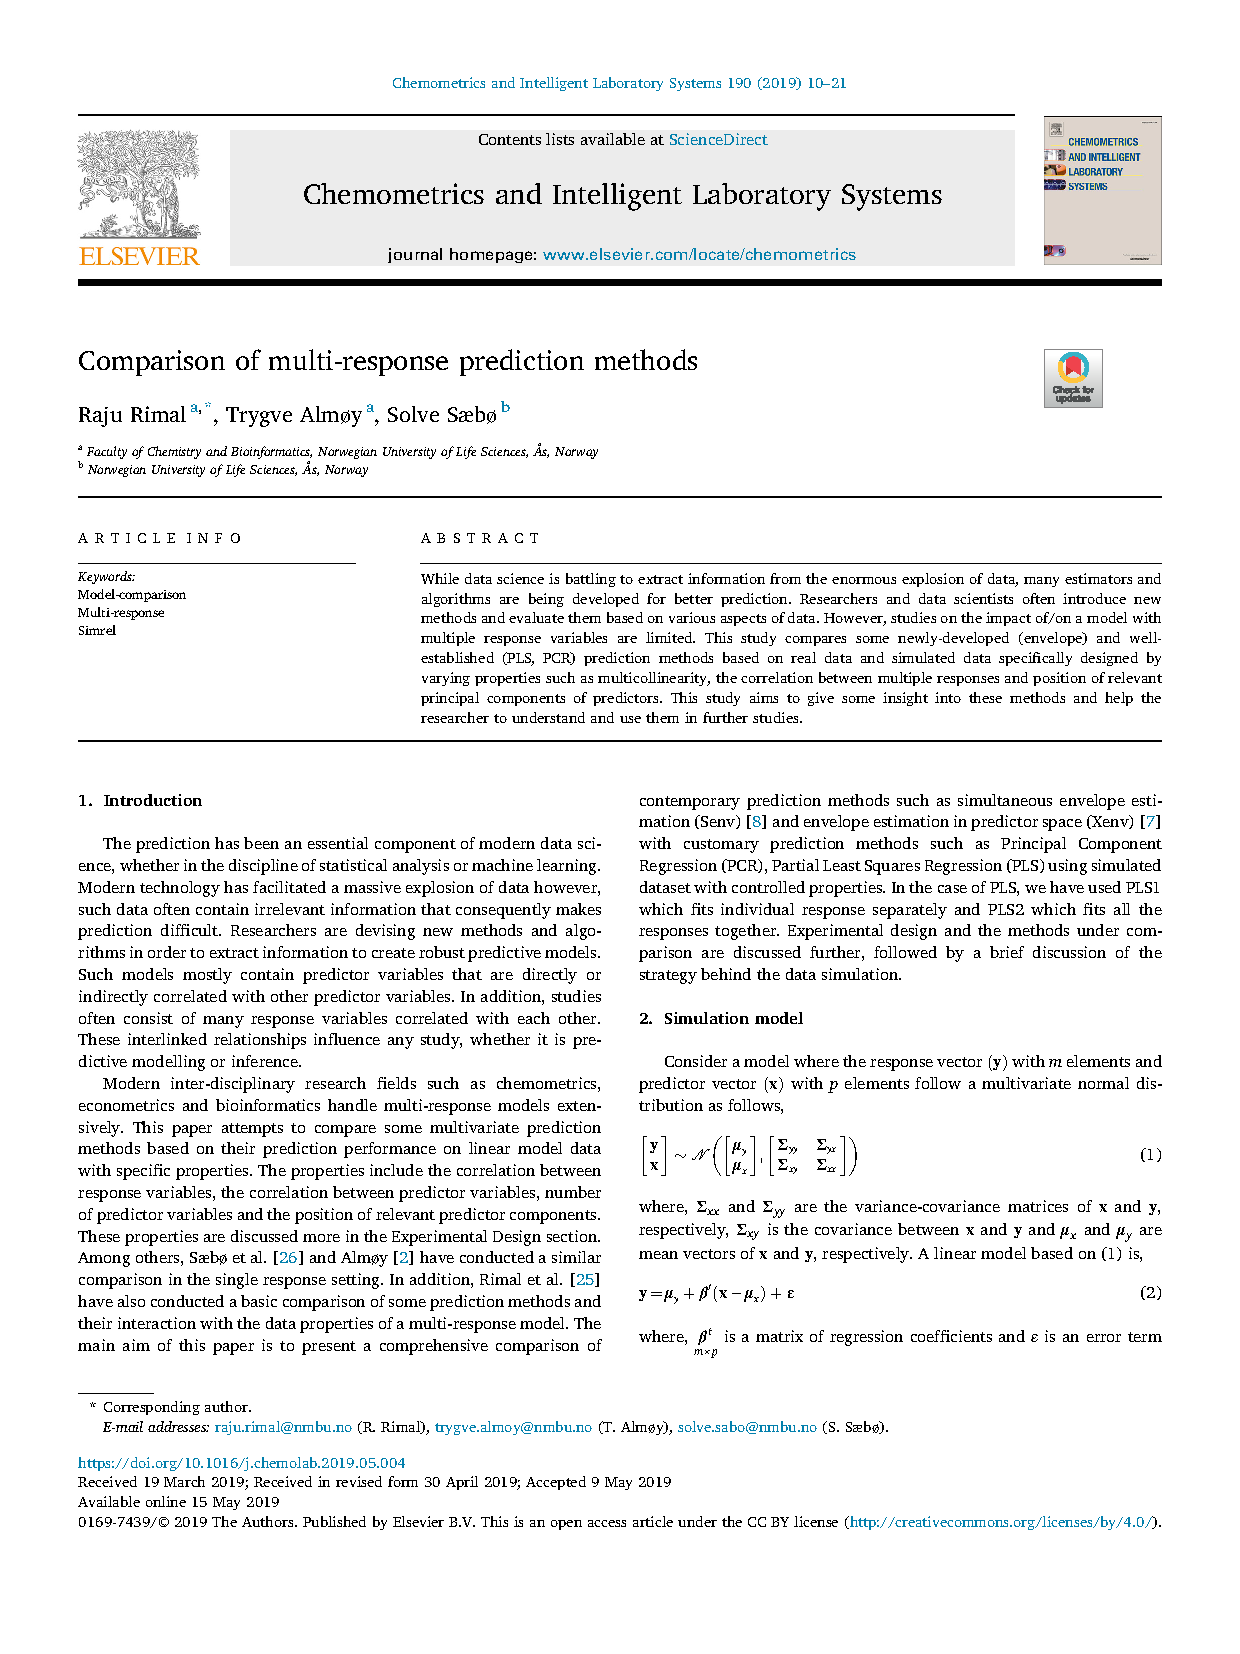
\includepdf[pages=-]{papers/003.pdf}
\par\chapter{Comparison of Multi-response Estimation Methods}
\cleardoublepage
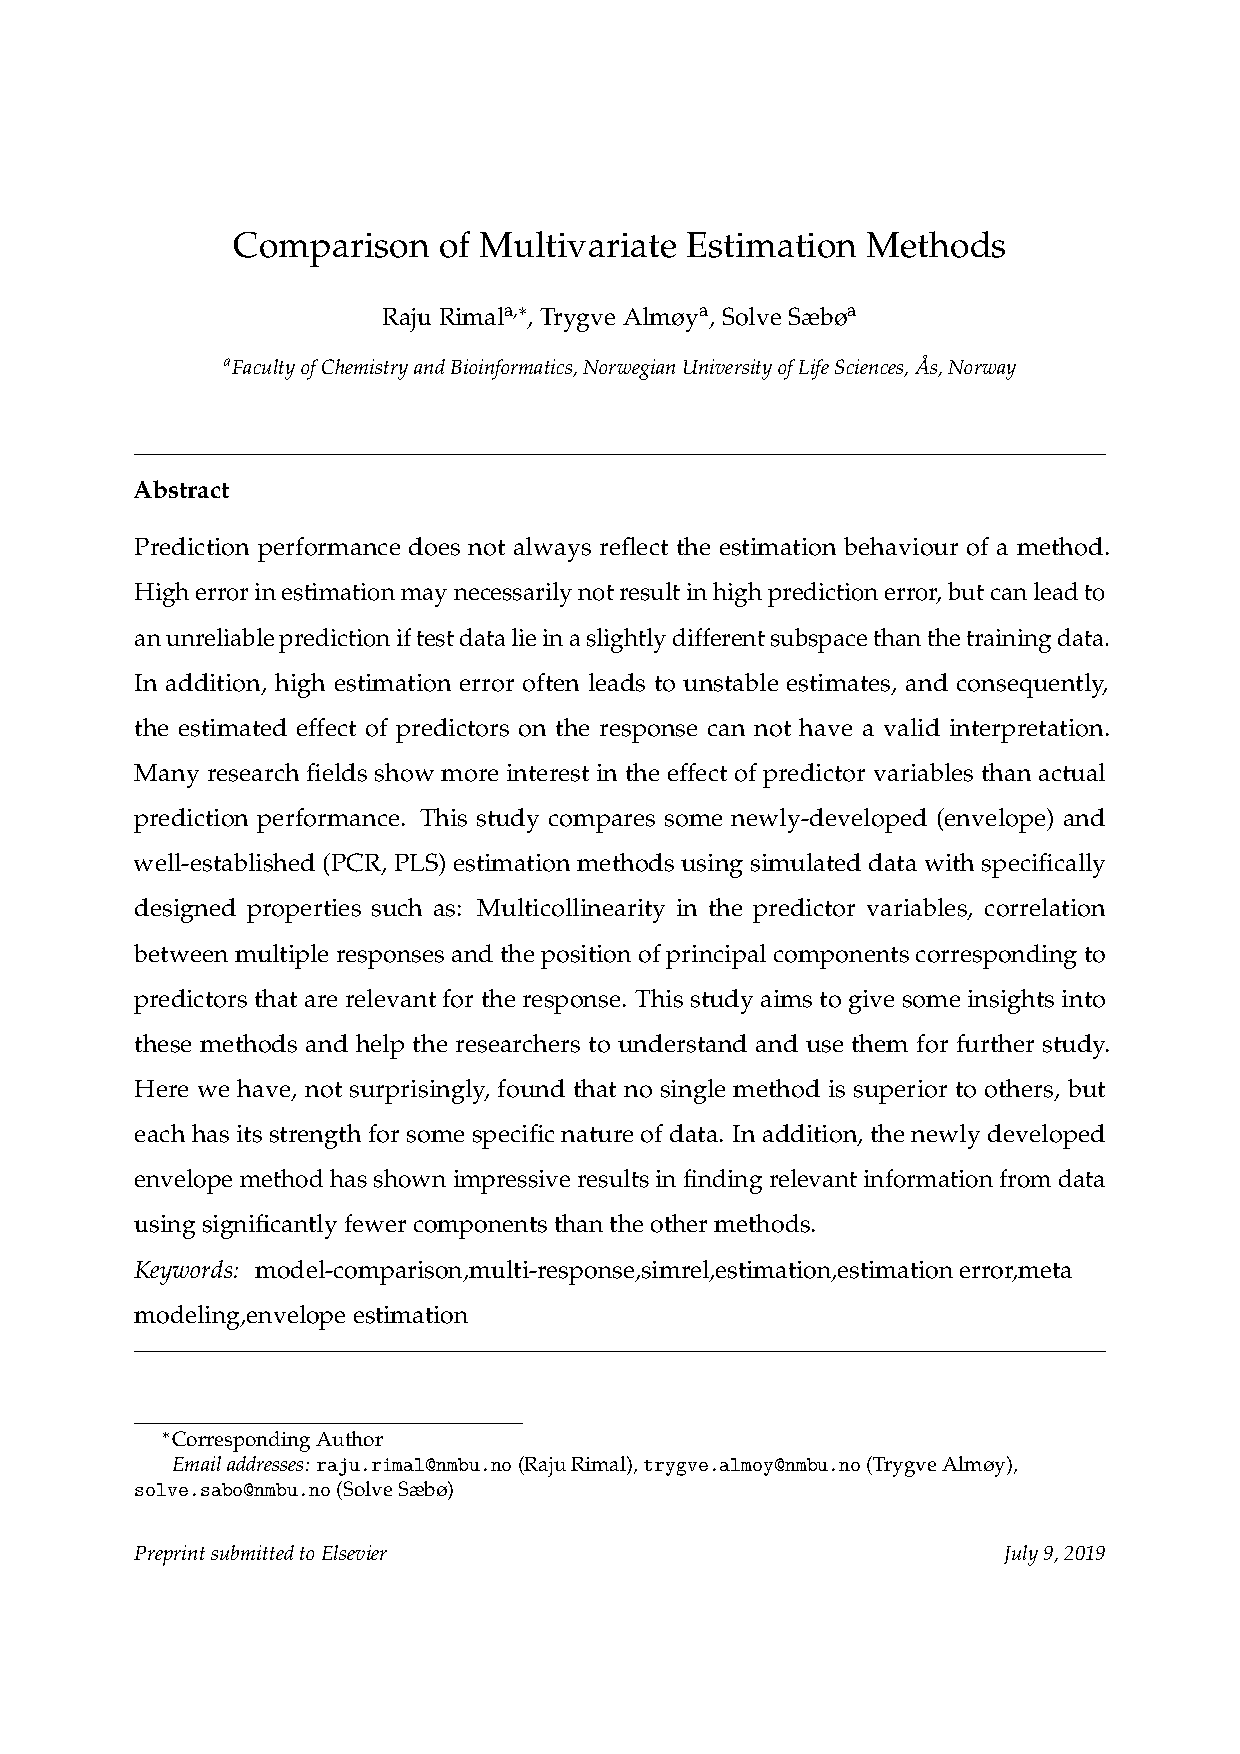
\includepdf[pages=-]{papers/004.pdf}

% *******************************************************
% ANYTHING EXTRA
% *******************************************************

\end{document}

%%% Local Variables:
%%% mode: latex
%%% TeX-master: t
%%% End:
